\section{GraphRule und Unvollständigkeit von RS-B2}

Die von Pellenkoft et al. entwickelten Regelsets, dienen als Grundlage für regelbasierte Optimierer wie Volcano. \cite{shanbhag2014optimizing} untersuchten sowohl die Vollständigkeit der vorgestellten Regel und fügten den bestehenden Regelsets ein neues hinzu, das alle andere Regelsets zum Join Reordering obsolet macht und zudem erheblich bessere Performance liefert.

Die Untersuchungen \cite{shanbhag2014optimizing} wurden mit dem Optimierer PyroJ durchgeführt. PyroJ ist ein Optimierer, der basierend auf Pyro \cite{roy2001multi} erstellt wurde und dem Volcano Optimizer nachempfunden ist. Zuerst wurden die Regelsets auf ihre Vollständigkeit hin geprüft. Neben der Prüfung auf Vollständigkeit konnte auch die neue Regel GraphRule Implementiert und so bzgl. ihrer Performance getestet werden.



\subsection{Implementierung von PyroJ}

PyroJ basiert auf dem von \cite{roy2001multi} in C++ Implementierten Optimierer Pyro und wurde automatisch von C++ nach Java übersetzt. Der Optimierer Pyro wurde nach dem Vorbild des Volcano Optimierers entwickelt. Volcano wurde als Vorbild gewählt, da es sich bei Volcano um einen hoch-repektierten, state-of-the-art, regelbasierten Optimierer handelt, der auch die Basis von kommerziellen Datenbanksytemen wie MS SQL Server ist. Außerdem ist Volcano, wie zuvor besprochen, hoch erweiterbar: Das Datenmodell, Executionmodell sind leicht erweiterbar, Transformationsregeln und Operatoren lassen sich hinzufügen. 

Einer der Unterschiede zwischen Volcano und Pyro ist die Trennung zwischen logical / physical Plan Generierung und der Suche nach dem optimalen Plan. Im Gegensatz zu Volcano werden erst alle logische Pläne für einen \ac{LQDAG} generiert, daraufhin werden dann alle Pläne in physische Pläne umgesetzt und basierend auf diesen Plänen der günstigste Plan ausgewählt.

Der Volcano Optimizer hingegen berechnet zuerst einen logischen Plan und generiert für diesen Plan dann alle physischen Pläne. Für diese Pläne wird der günstigste Plan gesucht. Die anderen Pläne müssen nicht mehr im Speicher vorgehalten werden. Daraufhin kann dann der nächste logische Plan generiert werden und die Kosten des günstigsten Plans mit dem bisher günstigsten Plan verglichen werden. Der Vorteil dieses Verfahrens ist, dass gerade bei großen Search Spaces der Plan im Speicher gehalten werden kann und suboptimale Pläne nicht länger als nötig gespeichert werden.

Genau wie das Volcano Projekt wird eine Memofunktion verwendet. \cite{roy2001multi} weist daraufhin, dass diese Memofunktion erst später dem Volcano Optimizer hinzugefügt wurde. Dadurch war es beispielsweise möglich, dass bei einer Anfrage, die aus $(A \Join B \Join C) \cup (B \Join C \Join D)$ zwei Äquivalenzknoten für den Knoten $B \Join C$ gebildet werden, obwohl alle Teilpläne von $A \Join B$ immer äquivalent sein werden und somit kein Grund besteht, die Pläne mehrfach zu berechnen. Pyro verwendet eine Memodatenstruktur, um die mehrfache Generierung des selben Teilplans zu unterbinden.

Ein weiterer Unterschied zu Volcano ist, dass es sich bei Pyro kein Optimizer generiert wird, sondern der Optimizer von vornherein in C++ geschrieben ist. Eine Übersetzung aus einem Description\-File hin zu C\-Code findet daher nicht statt.

\subsection{Getestete Regeln und Regelsets}

\cite{shanbhag2014optimizing} und \cite{roy2001multi} geben an, dass sie die Regelsets \textit{RS-B0}, \textit{RS-B1} und \textit{RS-B2} implementieren. Im Gegensatz zu Pellenkoft wird im Regelset \textit{RS-B1} nicht die Regel Swap verwendet, sondern Left\-Associtativity (vgl. \ref{PellenkoftVsPyro}). Beide Regeln sind jedoch semantisch ähnlich genug und können mit Hilfe von Kommutativität in einander überführt werden. Ebenfalls ist eine genaue Unterscheidung der Reihenfolge der Anwendung ähnlich wie bei Volcano nicht möglich. Alle Regeln laufen immer in einer vorgegeben Reihenfolge ab.

\begin{table}[ht]
\begin{tabular}{|l|l|l|}
\cline{1-3}
{\bf Regelmenge} & {\bf Pellenkoft}                                                                                                  & {\bf Pyro(J)}                                                                                                       \\ \cline{1-3}
{\bf RS-B0}   & \begin{tabular}[c]{@{}l@{}}Left Associativity\\ Right Associativity\\ Commutativity\end{tabular}            & \begin{tabular}[c]{@{}l@{}}Left Associativity\\ Right Associativity\\ Commutativity\end{tabular}              \\ \cline{1-3}
{\bf RS-B1 }  & \begin{tabular}[c]{@{}l@{}}Swap\\ Bottom Commutativity\end{tabular}                                         & \begin{tabular}[c]{@{}l@{}}Left Associativity\\ Commutativity\end{tabular}                                    \\ \cline{1-3}
{\bf RS-B2 }  & \begin{tabular}[c]{@{}l@{}}Left Associativity\\ Right Associativity\\ Commutativity\\ Exchange\end{tabular} & \begin{tabular}[c]{@{}l@{}}Left Associativity\\ Right Associativity\\ Commutativity\\ Exchange\end{tabular}   \\ \cline{1-3}
\end{tabular}
\caption{Unterschiede zwischen Pellenkoft und Pyro(J)}
\label{PellenkoftVsPyro}
\end{table}




\subsection{Unvollständigkeit von \textit{RS-B2}}



\begin{figure}[h]
  \centering
  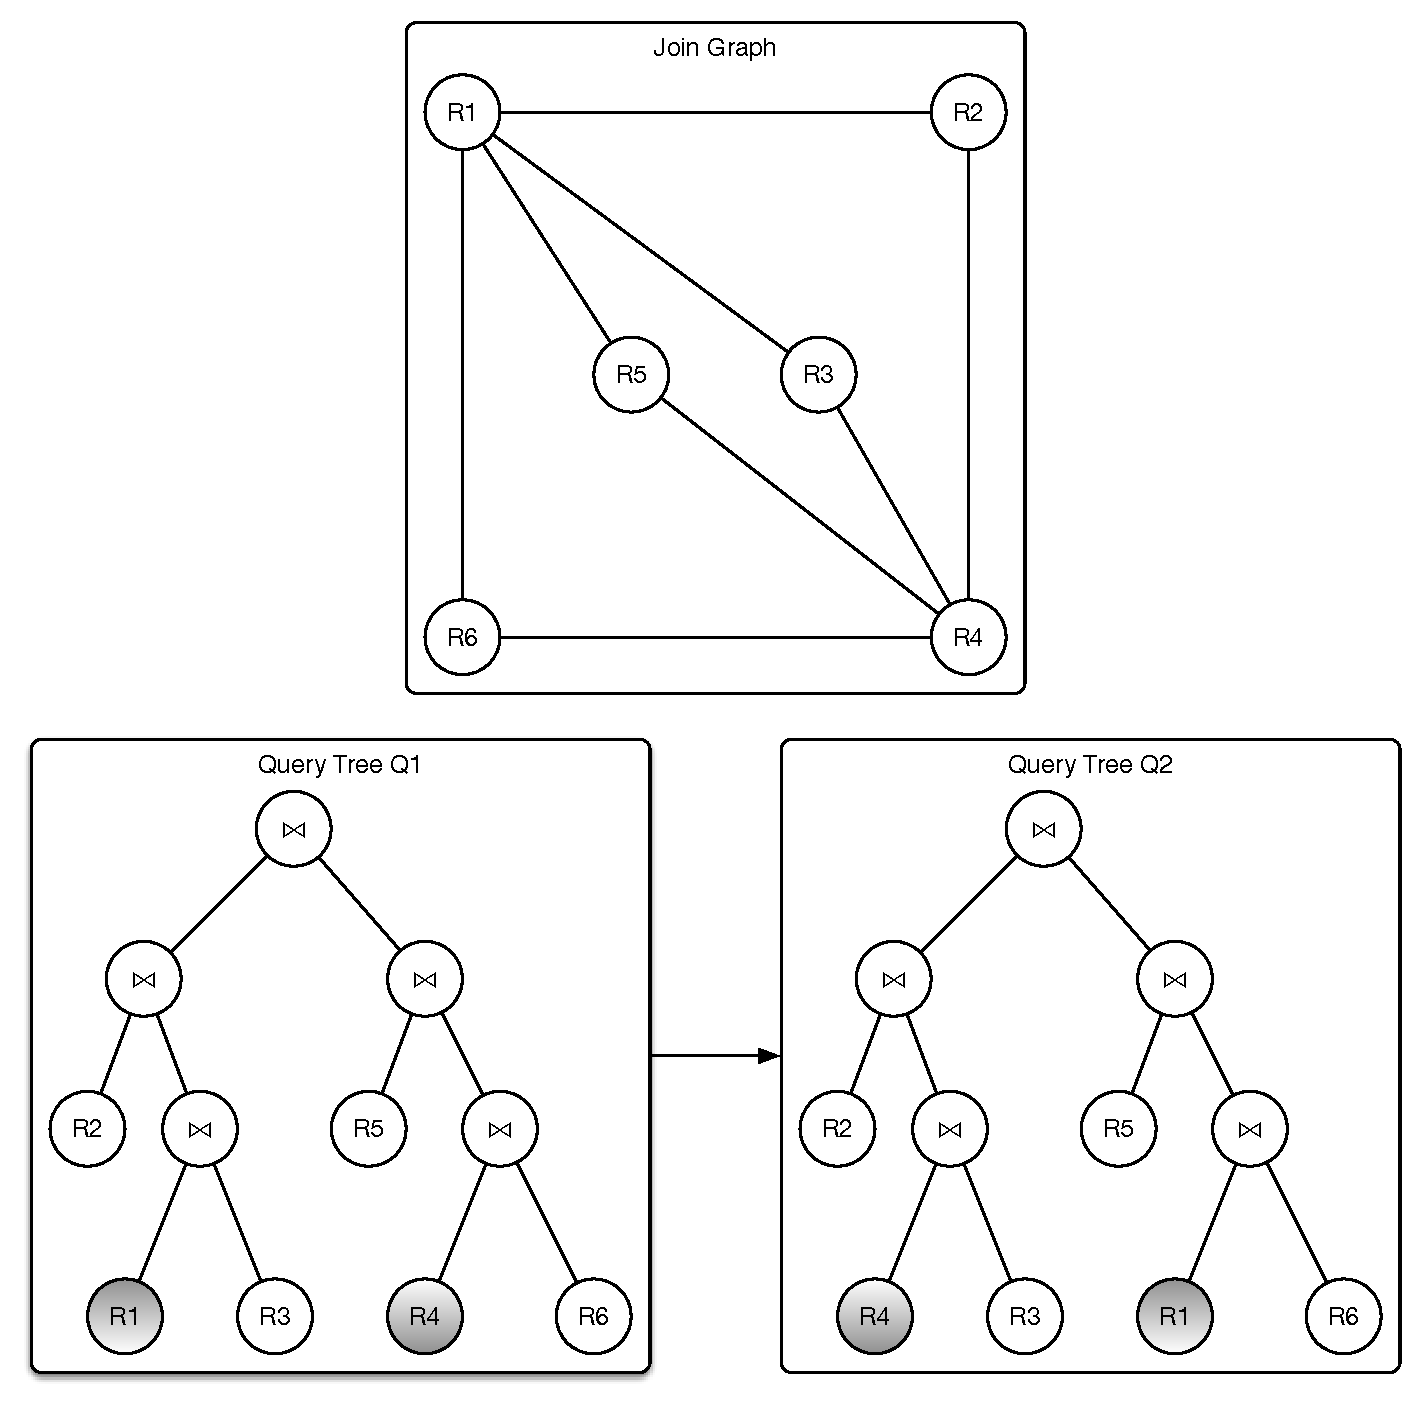
\includegraphics[width=\textwidth]{02_Related_Work/Graphs.pdf}
  \caption{Incompletness of RS-B2-CPS}
  \label{Incompleteness_RS-B2-CPS}
\end{figure}


Die Unvollständigkeit von \textit{RS-B2} wurde auf zwei Arten gezeigt. Auf der einen Seite wurde an Hand des Beispiel \ref{Incompleteness_RS} gezeigt. Im konkreten Beispiel sollte \textit{R1} und \textit{R4} getauscht werden. Wobei das Regelset \textit{RS-B2} zum Einsatz kommen sollte. Anhand des gegebenen Join Graphen ist die Transformation zwar Teil des Suchraums, kann jedoch durch die Regeln nicht erreicht werden. Das Regelset ist daher unvollständig.

Ebenfalls wurden unterschiedliche Abfragen mit Hilfe des Optimierers optimiert und geprüft, ob die selbe Menge an plänen aus den unterschiedlichen Regelsets entstehen kann. Wie zu erwarten war die Menge der Pläne, die aus \textit{RS-B0} nur \textit{RS-B1} entstanden sind gleich. Die Menge der \textit{RS-B2} Pläne stark reduziert. (vgl. \ref{tabelle)}.

Da nicht alle Pläne gefunden werden konnten, liegt es nahe, dass der optimale Plan möglicherweise nicht Teil des erforschten Suchraums ist. \cite{shanbhag2014optimizing} stellen fest, dass das Ergebnis mit \textit{RS-B2} erzeugt wurde bzgl. der berechneten Kosten um den Faktor 1.86 schlechter war, als die Pläne, die mit Hilfe eines vollständigen Regelsets erzeugt wurden. Wie genau die Zahl 1.86 zustande gekommen ist, ist nicht genauer begründet.

Es lässt sich also feststellen, dass mit Hilfe des Regelsets \textit{RS-B2} weniger Pläne im Suchraum gefunden werden konnten, als mit Hilfe des Regelsets \textit{RS-B1} bzw. \textit{RS-B2}. Ausserdem wurde festgestellt, dass Pläne aus unvollständigen Regelsets nicht immer den optimalen Plan beinhalten.





\subsection{Unvollständigkeit von RS\-02}




\cite{shanbhag2014optimizing} stellt fest, dass RS-B0-CPS und RS-B1-CPS vollständig sind. Die Vollständigkeit von RS-B2-CPS wird jedoch in Frage gestellt und die Unvollständigkeit mit Hilfe eines Beispiels belegt. Als Beispiel dient eine Menge von Relationen, die mit Hilfe des Jointrees J (\ref{fig:Incompleteness_RS-B2-CPS}) miteinander gejoint sind. Der Initale Anfragebaum \textit{Q1} ist in \ref{fig:Incompleteness_RS-B2-CPS} dargestellt. Das gewünschte Ergebnis nach einer Transformation \textit{Q2}  findet sich in \ref{fig:Incompleteness_RS-B2-CPS}. 

Bei \textit{RS-B2-CPS} dürfen die Regeln \textit{R2}, \textit{R3}, \textit{R4} nur jeweils einmal auf einen Join-Operator angewendet werden. Keine der Regeln darf danach auf den neu generierten Operator angewendet werden. Die In \ref{fig:Q1} und \ref{fig:Q2} zeichnet sich dadurch aus, dass die Relationen \textit{R1} und \textit{R4} vertauscht sind.


Die Vollständigkeit wurde auch mit Hilfe des PyroJ Optimierers geprüft. Hierbei wurde an Hand von Star-Queries  die Unvollständigkeit belegt. Wie in Abb. \ref{CompletenessResults} zu sehen, wurden mit Hilfe von \textit{RS-B2} nur knapp die Hälfte aller äquivalenten Pläne gefunden. Ebenfalls wird betont, dass die geschätzten Kosten des besten Plans, der durch \textit{RS-B2} erzeugt wurde um den Faktor 1.86 im Vergleich zu \textit{RS-B1} niedrigere geschätzte Kosten hatte.







\subsection{Vorschlag von RS-Graph}

\subsection{JOIN SETS}

Basierend auf dem bisherigen Wissen, wurden durch X und Y einige neue Begriffe festgelegt: W.
Ein Base Equivalence Knoten in einem expandierten LQDAG ist ein Äquivalenzknoten, der keinen Join Operator als Kinder hat. Ein solcher Knoten kann entweder eine Relation sein oder darf keine Join Operatoren als Kinder beinhalten.

Ein Join Tree ist in einem expandierten LQDAG ein Baum in der LQDAG dessen Wurzel ein Äuqivalenzknoten und jeder interne Knoten entweder ein Äquivalenzknoten oder ein Join Operator und jeder untergeordneter Knoten ein Äuqivalenzknoten ist.

Der Maximale JOIN Tree ist in einem expandierten LQDAG ein Join Tree, bei dem jeder Leaf Knoten ein Base Equivalence Node ist.

Ein Join-Set für einen Äquivalenzknoten E ist in einem expandierten LQDAG ein Paar $J = (S, P)$ bei dem S ein Set von Äquivalenzknoten ist, deren 

\subsection{Regelmenge RS-Graph}
Neben den bereits etablierten Regeln wird eine neue Regel für den Volcano Optimizer von \cite{shanbhag2014optimizing} vorgestellt. Die neue Transformationsregel \emph{RS-Graph} ersetzt die bisherigen Regeln und die bisherigen Regelsets. Die neue Regel erzeugt basierend auf einem Planknoten direkt alle möglichen äquivalenten Pläne. Somit sind alle Pläne unter einem bestimmten Äquivalenzknoten mit der Anwendung nur einer Regel erzeugt.

Die Regel \emph{RS-Graph} verwendet dazu die Subroutine $GraphRule$. Sie wird auf den Join Tree angewendet, falls die beiden mit einem Operator verbundenen Knoten A und B und deren Mitterknoten $P$. Für jedes Paar der J %\emph{equivalence nodes A,B and parent equivalence node P. For each pair of join-set (jsA,jsB) ∈ A.JoinSets∗B.JoinSets, we merge the pair to form a join-set js. We define the merge of the two join-sets jsA = (V1,P1) and jsB = (V2,P2) as (V1∪V2,P1 ∧P2).}

Um wiederholte Berechnungen des selben Join Trees zu vermeiden wird zudem geprüft, ob der Eltern-Äquivalenzknoten bereits $js$ beinhaltet. $$To check if two join- sets at an equivalence node are equal, it is sufficient to check if they have same equivalence nodes. If the join-sets have the same equivalence nodes, then they will also have the same predicates.$$

Für alle Join Sets $js$ des Parent nodes werden daraufhin zuerst alle JOIN partitionen gebildet bei denen $S_1 \Join S_2$ mit 

Sollte der $js$ noch nicht existieren, wird dieser dem JOIN Set hinzugefügt. Ein Graph wird basierend auf den $js$ gebildet, der mit Hilfe der Methode Partition in alle Partitionen getrennt wird. Aus denen werden wiederum Bäume erstellt, die an das Resultat zurückgegeben werden.

Die SubRoutine Create Graph, gibt ein JOIN Set, das JS einen Join Graphen aus, der




\subsection{Diskussion}
Die Implementierung der neuen Regel wurde in einem Java basierten regelbasierten Op den Äquivalenzklassen neue Felder hinzugefügt werden.

Die Generierung der Resultate findet ohne Pruning statt und Kosten für die Kostenberechnung werden nicht einbezogen. Ebenfalls bleiben Regeln bestehen, die für denn SELECT Pushdown verantwortlich sind, als Teil der Normalisierungsphase. 

Es wurden sowohl Star, Chain als auch Clique Queries getestet. Die Experimente fanden auf einem Intel i5 3.5 GHz mit 8 GB Ram statt. Es wurde festgestellt, dass die Geschwindigkeit der Optimierung verbessert werden konnte, dadurch, dass die Optimierung mehrfach durchgeführt wurde. Dieses Verhalten wurde auf Javas JIT Kompilierungsstrategie zurückgeführt, die erst den Code Kompiliert, wenn er auch tatsächlich gebraucht wird. Um sicherzustellen, dass der Kompilierte Code nicht wieder während der Ausführung vergessen wird, mussten spezielle Flags für die JVM gesetzt werden. Das Ergebnis war, dass die Dauer zwar verglichen zu den schnellsten Tests ohne das Flag langsamer, aber dafür konstant blieb.

Ebenfalls wurde bei Regelmenge $RS_B1$ geprüft, ob der gesamte Search Space erreicht wurde, indem die Anzahl der Äquivalenten Knoten und Operatoren im LQDAG gezählt wurden. Diese Zahl wurde mit der Zahl der Knoten in RS-Graph verglichen. Da beide Zahlen gleich waren, wird davon ausgegangen, dass beide Regelsets das selbe Ergebnis erzeugen. Eine Prüfung, die dies belegt fand aus technischen Gründen nicht statt.






Ersetzten X und Y die bisher gezeigten Regeln des Volcano Optimierers mit einer neuen Transformationsregel: RS-Graph. Die Regel kommt zur Anwendung, falls ein Graph dem Pattern $E_1 \Join E_2$ entspricht. Ist dies der Fall wird die Funktion $GraphRule(\Join, E_1, E_2, parent)$ aufgerufen. Sie erzeugt ein Set von allen Join Operatoren unter dem Äquivalenzklasse des $parent$-Knotens.







\subsection{Partition zu Graph}



Die Methode Partition gibt eine Menge von Partitionen zurück. Jede Partition bezeichnet eine Menge von Knoten. Sowohl $S_1$ als auch $G\\S_1$ sind Teil dieser Menge, falls beide zwischen beiden im Join-Graphen miteinander verbunden sind. Im Gegensatz zu anderen Regeln, die pro Anwendung der Regel nur immer einen neuen Knoten zurückgegeben haben, gibt die neue Regel immer Bäume zurück, die alle möglichen Join Operatoren unterhalb des ROOT Operators beinhalten.





Das bestehende Regel-Framework von Volcano wurde von \cite{shanbhag2014optimizing} mit einem neuen Regelset und einer neuen Regel erweitert. Das neue Regelset Graph Rule soll alle bestehenden Regeln zur JOIN-Tree Enumeration ersetzen. Im Gegensatz zu den vergleichsweise ineffektiven Regelsets, die bisher bekannt waren, setzt die neue Regel auf state-of-the-art, kreuzproduktfreie Join-Enumeratoren zur Suche nach äquivalenten Plänen. Damit kombiniert die neue Regel die Vorteile eines hoch erweiterbaren Systems wie Volcano mit der Geschwindigkeit von neuartigen Join-Enumeratoren.

Die neue Regel gibt nicht nur eine neue Variante des Query-Trees zurück, sondern bestimmt gleich auf einmal alle äquivalenten Pläne. Die Erweiterbarkeit des Volcano-Optimierers ermöglicht es auch eine solche komplexe, neue Regel zu implementieren.

Die neue Regel wird in drei Schritten umgesetzt. Zuerst werden die Subtrees bestimmt, auf die ein Paritionierungsalgorithmus im nächsten Schritt angewendet werden kann. Mit Hilfe der einzelnen Partitionen werden dann neue Bäume aufgebaut, die als alternative Pläne zurückgegeben werden. Diese drei Schritte sind auch in Abb. \ref{GraphRule} zu sehen.

\subsection{Routinen}





Um die Funktion der neuen Regel im Detail zu beschreiben, führt \cite{shanbhag2014optimizing} eine Reihe neuer Begriffe für einen Baum ein:

\begin{itemize}
\item \textit{Base Equivalence Node}: dieser Knoten bezeichnet einen Äuqivalenzknoten, der keine JOIN-Operatoren als dessen Kinder besitzt.
\item \textit{Join Equivalence Node}: dieser Begriff bezeichnet einen Äquivalenzknoten, der mindestens eine JOIN Operation untergeordnet hat.
\item \textit{Maximal Join Tree}: Dieser Baum ist ein Baum, der entweder Äquivalenzknoten oder einen JOIN Operator untergeordnet hat.
\item Ein \textit{Maximal join Tree} ist ein Baum, dessen Kinder immer EuqivalenceNodes sind.
\item Ein \textit{Join Set} für einen Äquivalenzknoten E ist ein Paar $J = (V, P)$ bei dem $V$ ein Set von Äquivalenknoten ist und deren Kinder seine 
\end{itemize}


\subsection{Implementierung}
Die Implementierung des neuen Regelsets wurde auf Basis des Query Optimierers PyroJ vorgenommen. PyroJ ist eine Übersetzung des in C++ entwickelten Optimierers Pyro, der an der Universität Bombay entwickelt wurde und das Volcano-Framework implementiert.

Alle Tests wurden auf einem Computer mit Intels Core i5 3.5 GHz mit 8 Gbyte Arbeitsspeicher und Ubuntu 11.10 durchgeführt. Die genaue Java Version und Einstellungen der JVM sind (fast) vollständig unbekannt.

Wie von \cite{shanbhag2014optimizing} beschrieben, wurde während er Performance Test festgestellt,dass sich die Dauer für die Ausführung einer Optimierung stark unterscheidet.Für die Durchführung einer Optimierung wurden zu Beginn erheblich höhere Werte festgestellt. Gerade die ersten Anfragen hatten eine besonders hohe Laufzeit. Erklärt wurde dieses Verhalten durch den Java \ac{JIT}-Compiler. Ebenfalls wurde erkannt, dass der Java eigene Code Optimierer HotSpot die Ergebnisse verfälschen kann. 

Während der Performance Tests wurde festgestellt, dass sich.........


\subsection{Probleme auf Grund der Plattformwahl}
Die Implementierung der neuen Regel wurde auf Basis von PyroJ vorgenommen. PyroJ ist eine Übersetzung des von ITT Bombay entwickelten Systems Pyro, das eine Implementierung des Volcano-Frameworks ist. PyroJ, das in Java implementiert ist, entstand durch eine automatische Konvertierung des C++ Codes von Pyro. 

Die Implementierung der Experimente wurde auf Basis von PyroJ vorgenommen. PyroJ ist eine Übersetzung des in C++ geschriebenen Query Optimierers Pyro nach Java. Der Optimierer wurde an der IIT Bombay gebaut und ist eine Implementierung des Volcano Optimization Frameworks.

Die Experimente wurden auf einem Intel Core i5 3.5 GHz Computer mit 8 Gbyte Arbeitsspeicher und Ubuntu 11.10 vorgenommen. Es wurde festegestellt, dass die Implementierung des Codes in Java verglichen zu C++ einigen Overhead generiert, der die Laufzeit der Optimierung negativ beeinflusst. Ebenfalls wurde festgestellt, dass die Laufzeit zur Optimierung einer Anfrage erheblichen Schwankungen unterlegen ist. Insbesondere konnten stark unterschiedliche Laufzeiten bei den selben Queries festgestellt werden. Queries, die zu Beginn ausgeführt wurden, wurden langsamer ausgeführt. Dieses Phänomen wurde auf den Java JIT-Compiler (HotSpot) zurückgeführt. Dieser Kompiliert nur die zur Ausführung notwendigen Teile des Programms und führt Optimierungen zur Laufzeit durch. Um konstante Laufzeiten für die selbe Anfrage zu erzielen, wurde nach eigenen angaben die JIT-Kompilierung ausgeschaltet. Außerdem wurde das Java HotSpot JVM flag $-XX:CompileThreshold=1$ gesetzt und einige große Queries ein paar mal optimiert, um sicherzustellen, dass alle Funktionen auch kompiliert werden bevor sie ausgeführt werden.
 

\subsection{Kritik} \todo{Wo soll dieser Teil eigentlich hin? Evaulation/ Related Work / Implementierung}


Die Implementierung des Frameworks wirft einige Fragen auf. Auf der einen Seite wird durch den Autor selbst festgestellt, dass durch die Wahl einer anderen Code Basis (C++ statt Java) Ergebnisse mit weniger Overhead erzielt werden könnten. Warum also die Entscheidung zur Implementierung in Java gefallen ist, bleibt unbeantwortet.

Auch die Probleme, die durch den JIT Compiler entstanden sind, sind außergewöhnlich. Zuerst wurde die Kompilierung nach eigenen Angaben abgeschaltet und dann wiederum sichergestellt, dass alles kompiliert wurde indem große Anfragen optimiert wurden. Was genau mit dieser Aussage gemeint ist bleibt unbeantwortet.  Ich nehme an, dass nur das JVM Flag $-XX:CompileThreshold=1$ gesetzt wurde. Dieses Flag gibt an, nach wie vielen Methodenaufrufen ein Stück Java Code in Maschinencode kompiliert wird. Der Standardwert liegt bei 10000 \cite{oracle2015VMOptions}. Dank dieses Flags wird bereits beim ersten Aufruf einer Methode die Methode auch kompiliert. Warum dieser Umweg gewählt wurde, bleibt wage.

Ein weiterer Grund für Fehler bei der Messung kann die Wahl der Plattform im Allgemeinen sein. Da die Ausführung des Programms zu jedem beliebigen Zeitpunkt durch die Garbage Collection unterbrochen werden kann, können Messungen der Laufzeit nur schwer vorgenommen werden. Um wenigstens einen Hinweis auf diese Messfehler zu finden, wäre eine Nutzung der JVM Flags $ -verbose:gc -XX:+PrintGCDateStamps -XX:+PrintGCDetails$ möglich gewesen. Diese Flags geben an, wann die Garbage Collection zuschlägt und wieviel Zeit diese zur Ausführung benötgt. \cite{andreasson2015JVM}  


Warum also trotz all dieser möglichen Fehlerquellen und Ungenauigkeiten gerade Java zum Einsatz gekommen ist, ist unklar und wenig verständlich. Insbesondere da eine Alternative in C++ mit Pyro bereitstand.


